\iffalse

MIT License

Copyright (c) 2023-2025 Aron Hardeman

Permission is hereby granted, free of charge, to any person obtaining a copy
of this software and associated documentation files (the "Software"), to deal
in the Software without restriction, including without limitation the rights
to use, copy, modify, merge, publish, distribute, sublicense, and/or sell
copies of the Software, and to permit persons to whom the Software is
furnished to do so, subject to the following conditions:

The above copyright notice and this permission notice shall be included in all
copies or substantial portions of the Software.

THE SOFTWARE IS PROVIDED "AS IS", WITHOUT WARRANTY OF ANY KIND, EXPRESS OR
IMPLIED, INCLUDING BUT NOT LIMITED TO THE WARRANTIES OF MERCHANTABILITY,
FITNESS FOR A PARTICULAR PURPOSE AND NONINFRINGEMENT. IN NO EVENT SHALL THE
AUTHORS OR COPYRIGHT HOLDERS BE LIABLE FOR ANY CLAIM, DAMAGES OR OTHER
LIABILITY, WHETHER IN AN ACTION OF CONTRACT, TORT OR OTHERWISE, ARISING FROM,
OUT OF OR IN CONNECTION WITH THE SOFTWARE OR THE USE OR OTHER DEALINGS IN THE
SOFTWARE.

\fi\section{Differentiation \& integration}
\subsection{Differentiation}
\tableofcontents[currentsection,currentsubsection]
\begin{frame}

\frametitle{Basic differentiation}

\begin{itemize}
\item  Differentiation is usually easy, thus we will only include some examples without explaining all rules first. (One exception is differentiating $x^x$ which will be covered in more detail.)
\pause\item Example: $[\ln(2x^2-3x+4)]'=\frac{[2x^2-3x+4]'}{2x^2-3x+4}=\frac{4x-3}{x^2-3x+4}$
\pause\item Example: $\frac{d}{dx}(3) = 0$
\pause\item Example: $(2x+1)^{7}=14(2x+1)^6$ (do not expand brackets, but use the chain rule instead) 
\pause\item Example: $\frac{d^4(\sin x)}{dx^4}=\frac{d^3(\cos x)}{dx^3}=\frac{d^2(-\sin x)}{dx^2}=\frac{d(-\cos x)}{dx}=\sin x$
\pause\item Therefore also: $\sin x = \frac{d^4(\sin x)}{dx^4} =  \frac{d^8(\sin x)}{dx^8} =  \frac{d^{12}(\sin x)}{dx^{12}}=  \hdots=\frac{d^{400}(\sin x)}{dx^{400}}=\hdots$

(This is useful when computing the Taylor series of $\sin x$.)
\end{itemize}


\end{frame}

\begin{frame}

\frametitle{Differentiation example}
\begin{flalign*}
\action<+->{\hspace{-4mm}\frac{d}{dx}\sin\left(\frac{e^{x^3}}{3x^2}\right)&=\left[\frac{e^{x^3}}{3x^2}\right]'\cos\left(\frac{e^{x^3}}{3x^2}\right)=\frac{3x^2[e^{x^3}]'-e^{x^3}[3x^2]'}{(3x^2)^2}\cos\left(\frac{e^{x^3}}{3x^2}\right)\\[-0.5 ex]}
\action<+->{&=\frac{3x^2(e^{x^3}[x^3]')-6xe^{x^3}}{(3x^2)^2}\cos\left(\frac{e^{x^3}}{3x^2}\right)\\[-0.5 ex]}
\action<+->{&=\frac{3x^2(3x^2 e^{x^3})-6xe^{x^3}}{(3x^2)^2}\cos\left(\frac{e^{x^3}}{3x^2}\right)\\[-0.5 ex]}
\action<+->{&=\boxed{e^{x^3}\left(1-\frac{2}{3x^3}\right)\cos\left(\frac{e^{x^3}}{3x^2}\right)}\\[-0.5 ex]}
\end{flalign*}


\end{frame}

\begin{frame}

\frametitle{A  trick to differentiate $x^x$}

\begin{itemize}
\item  We know how to differentiate $[c^x]'=c^x\ln c$ as well as $[x^c]'=cx^{c-1}$. But what if $x$ appears in both the base and the exponent?

\pause
\item Let $y(x)=x^x$. \pause Then $y=(e^{\ln x})^x$ \pause $=e^{x\ln x}$

The derivative then becomes: $y'(x)=e^{x\ln x}\cdot[x\ln x]'$

Which is equal to $\boxed{y'(x)=x^x(1+\ln x)}$

\pause\item Alternatively, use the following method: $y=x^x$

Taking the logarithm: $\ln y = \ln(x^x)$\pause $ =x\ln x$ 

\pause
Implicit differentiation: $\frac{y'}{y} = 1 + \ln x$\hspace{10mm} {\small(Why not $\frac{1}{y}$?)}

\pause
Multiply both sides with $y=x^x$: $\boxed{y'(x)=x^x(1+\ln x)}$

\pause\item Analogous reasoning can be used to differentiate similar functions like $(2x)^{5x+1}$.
\end{itemize}


\end{frame}

\begin{frame}

\frametitle{Differentiating $f(x)^{g(x)}$}

We could create a ``power rule" for functions, similar to the product rule, quotient rule etc.

So, say we have two functions $f=f(x)$ and $g=g(x)$, and that $y(x)=f(x)^{g(x)}$ Then we have:\pause
\begin{flalign*}
\action<+->{&y=f^g=(e^{\ln f})^g=e^{g\ln f}\\}
\action<+->{&y'=e^{g\ln f}[g\ln f]'=f^g[g\ln f]'\\}
\action<+->{&y'=f^g\left({g\frac{f'}{f}+g'\ln f}\right)\\}
\end{flalign*}
\action<+->{ So our ``power rule" turns out to be \[\boxed{[f^{g}]'=f^g\left({g\frac{f'}{f}+g'\ln f}\right)}\]}

\end{frame}

\subsection{Integration \& Applications}
\tableofcontents[currentsection,currentsubsection]
\begin{frame}
\frametitle{Integration: simple integrals}
\begin{itemize}
\item $\int xdx = \frac{1}{2}x^2+C$
\pause\item $\int \cos (x)dx = \sin(x)+C$
\pause\item $\int_2^3 (\frac{1}{x} + \frac{1}{x^2})dx=[\ln|x|-\frac{1}{x}]_2^3=(\ln(3)-\frac{1}{3})-(\ln(2)-\frac{1}{2})=\ln(\frac{3}{2})+\frac{1}{6}$
\pause\item Do not forget to write $+C$ for indefinite integrals!
\end{itemize}
\end{frame}

\begin{frame}
\frametitle{Integration basics}
\begin{itemize}
\item Sometimes, you see both a function and a function's derivative in the same integral. Sometimes you can then use the chain rule in the opposite direction, as follows:
\pause\item $\int \frac{\cos x}{\sin x} dx =$\pause$ \int \frac{1}{\sin x}[\sin x]'dx= \ln\left|\sin x\right|+C$
\pause\item $\int e^x\sin(100+3e^x)dx=$\pause$\frac{1}{3}\int [100+3e^x]'\sin(100+3e^x)dx=-\frac{1}{3}\cos(100+3e^x)+C$
\pause\item $\int\frac{xdx}{x^2+137}=$\pause$\frac{1}{2}\int\frac{2xdx}{x^2+137}=\frac{1}{2}\int\frac{[x^2+137]'dx}{x^2+137}=\frac{1}{2}\ln\left|x^2+137\right|+C$
\pause\item These integrals can also be solved using a substitution.
\end{itemize}
\end{frame}

\begin{frame}{Substitution rule (1)}
    \begin{itemize}
        \item The integrals from the last slide can also be solved using substitution.
        \item Example: $\int\frac{xdx}{x^2+137}$
        \pause\item When we set $u=x^2+137$, we find $du=2xdx$, thus:
        \pause\item $\int\frac{xdx}{x^2+137}=\frac{1}{2}\int\frac{1}{u}du=\frac{1}{2}\ln|u|+C=\frac{1}{2}\ln|x^2+137|+C$
        \pause\item Do not forget to convert the $u$ back to $x$!        
    \end{itemize}
\end{frame}

\begin{frame}{Substitution rule (2) }
    \begin{itemize}
        \item Question: calculate $\int\frac{(\ln x)^2}{x}dx$
        \item\pause Detailed solution: we observe that $[\ln x]'=\frac{1}{x}$, and we also see that $\frac{1}{x}$ appears in our integral. Thus, let us try $u=\ln x$.
        \item\pause Then $du=\frac{1}{x}dx$, and therefore \[\int\frac{(\ln x)^2}{x}dx=\int u^2 du=\frac{1}{3}u^3+C = \boxed{\frac{1}{3}(\ln x)^3+C}\]
        \item\pause {\footnotesize (It takes practice to find good substitutions.)}
    \end{itemize}
\end{frame}

\begin{frame}
\frametitle{Integration by parts (1)}{\small
\vspace{-3mm}\begin{tcolorbox}[colback=yellow!50,colframe=violet!75!black,title=General form -- Integration By Parts]
{\small Indefinite integrals: $\int \textcolor{red}{u(x)}\textcolor{blue}{v'(x)}dx=[\textcolor{red}{u(x)}\textcolor{blue}{v(x)}]-\int \textcolor{red}{u'(x)}\textcolor{blue}{v(x)}dx$

Definite integrals: $\int_a^b \textcolor{red}{u(x)}\textcolor{blue}{v'(x)}dx=[\textcolor{red}{u(x)}\textcolor{blue}{v(x)}]_a^b-\int_a^b \textcolor{red}{u'(x)}\textcolor{blue}{v(x)}dx$}
\end{tcolorbox}
\begin{itemize}
    \item\pause $\int \textcolor{red}{x}\textcolor{blue}{\cos x} dx = [\textcolor{red}{x}\textcolor{blue}{\sin x}] - \int \textcolor{red}{1}\cdot\textcolor{blue}{\sin x} dx = x\sin x + \cos x + C$
    \item\pause $\int \textcolor{red}{x}\textcolor{blue}{e^{3x}} dx=[\textcolor{red}{x}\cdot\textcolor{blue}{\frac{1}{3}e^{3x}}]-\int \textcolor{red}{1}\cdot\textcolor{blue}{\frac{1}{3}e^{3x}} dx=\frac{1}{3}xe^{3x}-\frac{1}{9}e^{3x}+C$
    \item We see from examples 1 and 2 that if we have x in front of something we know how to integrate, then we can also integrate the new thing! However, ``I.B.P." is more powerful than that.
\end{itemize}
}\end{frame}

\begin{frame}
\frametitle{Integration by parts (2)}{\small
\vspace{-3mm}\begin{tcolorbox}[colback=yellow!50,colframe=violet!75!black,title=General form -- Integration By Parts]
{\small Indefinite integrals: $\int \textcolor{red}{u(x)}\textcolor{blue}{v'(x)}dx=[\textcolor{red}{u(x)}\textcolor{blue}{v(x)}]-\int \textcolor{red}{u'(x)}\textcolor{blue}{v(x)}dx$

Definite integrals: $\int_a^b \textcolor{red}{u(x)}\textcolor{blue}{v'(x)}dx=[\textcolor{red}{u(x)}\textcolor{blue}{v(x)}]_a^b-\int_a^b \textcolor{red}{u'(x)}\textcolor{blue}{v(x)}dx$}
\end{tcolorbox}
\begin{itemize}
    \item Example: $\int \log_2(3w^{w^4})dw
    =
    \frac{1}{\ln2}\int (\ln(3) +w^4 \ln (w))dw
    =
    \frac{\ln3}{\ln2}w + \frac{1}{\ln2}\int \textcolor{red}{\ln(w)}\cdot \textcolor{blue}{w^4}dw
    =
    \frac{\ln3}{\ln2}w +\frac{1}{\ln2}\left({[\textcolor{red}{\ln(w)}\cdot\textcolor{blue}{\frac{1}{5}w^5}]-\int\textcolor{red}{\frac{1}{w}}\cdot\textcolor{blue}{\frac{1}{5}w^5}dw}\right)
    =
    \frac{\ln3}{\ln2}w +\frac{1}{\ln2}\left({[\frac{1}{5}w^5\ln(w)]-\int\cdot\frac{1}{5}w^4dw}\right)
    =
    \frac{\ln3}{\ln2}w +\frac{1}{\ln2}\left({\frac{5}{25}w^5\ln(w)-\frac{1}{25}w^5}\right)+C
    =
    \boxed{\mathsmaller{\frac{\ln3}{\ln2}w +\frac{1}{25\ln2}\left({5w^5\ln(w)-w^5}\right)+C}}$

\end{itemize}
}\end{frame}

\begin{frame}[label=current]
\frametitle{Repeated integration by parts}\vspace{-2.2mm}
\begin{itemize}
    {\small\item We saw that if we have something we can integrate (say $\sin x$ or $e^x$), then we can also integrate the product of that function with $x$ (so we can integrate $x\sin x$ or $xe^x$).
    \item\pause By applying I.B.P multiple times, we can even work away higher powers of $x$:
    \pause\item Question: integrate $\int x^3\sin (x)dx$.
    \pause\item Solution (pay attention to plus/minus!):}
    \vspace{-2mm}\begin{flalign*}
        \hspace{-12mm}\int x^3&\sin (x)dx = [-x^3\cos x]+3\int x^2\cos (x)dx\\[-1.3 ex]
        \action<+->{&= [-x^3\cos x]+3\left([x^2\sin x]-2\int x\sin(x) dx\right)\\[-0.9 ex]}
        \action<+->{&= [-x^3\cos x]+3\left([x^2\sin x]-2\left({[-x\cos x]+\int\cos(x)dx}\right)\right)\\[-0.9 ex]}
        \action<+->{&= [-x^3\cos x]+3\left([x^2\sin x]-2\left({[-x\cos x]+\int\cos(x)dx}\right)\right)\\[-0.9 ex]}
        \action<+->{&=-x^3\cos x +3x^2\sin x +6x\cos x-6\sin x + C}
    \end{flalign*}
\end{itemize}
\end{frame}

\begin{frame}
\frametitle{Solving $\int e^x\sin (x)dx$ and $\int e^x\cos (x)dx$ with I.B.P.}\vspace{-2.2mm}
\begin{itemize}
    \item Question: find $\int e^x\sin (x)dx$.
    \pause\item Solution:
    \begin{flalign*}
        \action<+->{\textcolor{violet}{\int e^x}&\textcolor{violet}{\sin(x)dx}=[e^x\sin x]-\int e^x\cos(x)dx}\\
        \action<+->{&=e^x\sin x-\left({[e^x\cos x]+\int e^x\sin(x)dx}\right)}\\
        \action<+->{&=e^x\sin x-{e^x\cos x-\textcolor{violet}{\int e^x\sin(x)dx}}}
    \end{flalign*}
    \action<+->{ We can now add $\textcolor{violet}{\int e^x\sin(x)dx}$ to both sides:
    \[\hspace{-16mm}2\textcolor{violet}{\int e^x\sin(x)dx}=e^x(\sin x-\cos x)+C\]}\action<+->{\[\vspace{0mm}\implies\boxed{{\textcolor{black}{\int e^x\sin(x)dx}=\frac{1}{2}e^x(\sin x-\cos x)+C_*}}\quad\text{(where $C_*=\frac{1}{2}C$)}\]}
    
\end{itemize}
\end{frame}

\begin{frame}{Trigonometric substitutions: example (slide 1)}
    \begin{itemize}
        \item Question: find \[\int_2^5 \frac{\sqrt{x^2-4}}{x^3}dx\]
        \pause\item Solution: we substitute $x=2\sec\theta$ (for $0\leq\theta<\pi/2$ or $\pi\leq\theta<3\pi/2$). It will be explained later why we choose this substitution. Then we have $dx=2\sec \theta\tan \theta d\theta$.\pause We find: \begin{flalign*}
            \sqrt{x^2-4}&=\sqrt{(2\sec\theta)^2-4}=2\sqrt{\sec^2\theta-1}=2\sqrt{\tan^2 \theta}\\
            &=2\left|\tan\theta\right|=2\tan \theta
        \end{flalign*}
        (We know that $2\left|\tan\theta\right|=2\tan \theta$ because $\tan \theta\geq0$ for $0\leq\theta<\pi/2$ or $\pi\leq\theta<3\pi/2$)

        \pause Integral bounds: if $x=2\sec\theta=2$ then $\theta=0$. If $x=2\sec\theta=5$ then $\theta=\arccos(\frac{2}{5})$. The integral will be worked out in the next slide.
    \end{itemize}
\end{frame}
% ={\frac{\arccos(\frac{2}{5})}{2}-\frac{1}{4}\sin(2\arccos(\frac{2}{5}))}

\begin{frame}{Trigonometric substitutions: example (slide 2)}
        \action<+->{Integral bounds: if $x=2\sec\theta=2$ then $\theta=0$. If $x=2\sec\theta=5$ then $\theta=\arccos(\frac{2}{5})$. So, we have:} \begin{flalign*}
            \action<+->{\int_2^5 &\frac{\sqrt{x^2-4}}{x^3}dx=\int_0^{\arccos(2/5)}\frac{2\tan\theta}{8\sec^3\theta}2\sec \theta\tan \theta d\theta}\\
            \action<+->{&=\frac{1}{2}\int_0^{\arccos(2/5)}\sin^2\theta d\theta=\frac{1}{2}\int_0^{\arccos(2/5)}\left(\frac{1}{2}-\frac{1}{2}\cos2\theta\right) d\theta\\}
            &\action<+->{=\frac{1}{2}\left[\frac{\theta}{2}-\frac{1}{4}\sin2\theta\right]_0^{\arccos(2/5)}}
            \action<+->{=\boxed{{\frac{\arccos(\frac{2}{5})}{4}-\frac{1}{8}\sin\left(2\arccos\left(\frac{2}{5}\right)\right)}}\\}
            \action<+->{&\textcolor{lightgray}{={\frac{\arccos(\frac{2}{5})}{4}-\frac{1}{8}\left(2\sin\left(\arccos\left(\frac{2}{5}\right)\right)\cos\left(\arccos\left(\frac{2}{5}\right)\right)\right)}}\\
            &\textcolor{lightgray}{={\frac{\arccos(\frac{2}{5})}{4}-\frac{1}{10}\sin\left(\arccos\left(\frac{2}{5}\right)\right)}=\boxed{{\frac{\arccos(\frac{2}{5})}{4}-\frac{\sqrt{21}}{50}}}}}
        \end{flalign*}
\end{frame}

\begin{frame}{Trigonometric substitutions table}
    \begin{itemize}
        \item In the previous example, we substituted $x=2\sec\theta$ and everything magically worked out. How did we find this substitution? Well, we used this scheme:
        \end{itemize}

        \begin{tcolorbox}[colback=yellow!50,colframe=violet!85!black,title=Trigonometric substitutions for integration]
            \centering
        \begin{tabular}{ |c|c|c| } 
         \hline
         Expression & Use the substitution & And use \\
         \hline\hline&&\\[-2.2ex]
         $\sqrt{a^2-x^2}$ & $x=a\sin\theta$, $-\frac\pi2\leq\theta\leq\frac\pi2$ & $1-\sin^2\theta=\cos^2\theta$ \\ 
         $\sqrt{a^2+x^2}$ & $x=a\tan\theta$, $-\frac\pi2<\theta<\frac\pi2$ &  $1+\tan^2\theta=\sec^2\theta$ \\ 
         $\sqrt{x^2-a^2}$ & $x=a\sec\theta$, {\footnotesize$0\leq\theta<\frac\pi2$ or $\pi\leq\theta\frac{3\pi}2$} &  $\sec^2\theta-1=\tan^2\theta$\\ 
         \hline
         
        \end{tabular}
        
        \end{tcolorbox}
    
\end{frame}

\begin{frame}{Watch out!}
    \begin{itemize}
        \item Question: solve \[\int t\sqrt{t^2+2}dt\]
        \item\pause Observation: we recognize that this integral contains the term $\sqrt{t^2+2}$, thus we could try to make a trigonometric substitution. \pause However, this is going to cost much time.

        It is much easier to say: $u=t^2+2$, so $du=2tdt$ and solve the integral that way, without any need for ``trig sub".

        \pause\item So, please think twice and be sure that no other way works, before doing trig substitution!
    \end{itemize}
\end{frame}

\begin{frame}{Integration by partial fractions}
    Sometimes you want to integrate the quotient of two polynomials: \[f(x)=\frac{P(x)}{Q(x)}\].

    \pause
    Assume for now (\textbf{very important!}) that the degree of $P$ is lower than the degree of $Q$ (otherwise do long division first).

    \pause
    Then we compute the integral as follows:
    \begin{enumerate}
        \item Write $f(x)$ as a \emph{sum} of terms (\emph{partial fractions}) of the form $\frac{A}{(ax+b)^i}$ and $\frac{Ax+B}{(ax^2+bx+c)^j}$ (see next slide).
        \pause\item Solve for the constants $A$, $B$, $\dots$.
        \pause\item Integrate each partial fraction.
    \end{enumerate}
\end{frame}

\begin{frame}{Finding the partial fraction decomposition}
    We have $f(x)=\frac{P(x)}{Q(x)}$ \underline{(where $\mathop{\text{deg}}(P)<\mathop{\text{deg}}(Q)$)}. The goal is to write $f(x)$ as a sum of partial fractions.

    \begin{enumerate}
        \pause\item If $Q(x)=(a_1x+b_1)(a_2x+b_2)\dots(a_kx+b_k)$ is the product of distinct linear factors, then there exist constants $A_1,\dots,A_k$ s.t. $\frac{P(x)}{Q(x)}=\frac{A_1}{a_1x+b_1}+\frac{A_2}{a_2x+b_2}+\dots+\frac{A_k}{a_kx+b_k}$.
        \pause\item If some linear factor is repeated, it will occur multiple times in the partial fraction decomposition: if we have $Q(x)=\hdots\cdot(a_ix+b_i)^r\cdot\dots$, we get $\frac{P(x)}{Q(x)}=\hdots+\left(\frac{A_1}{a_ix+b_i}+\frac{A_2}{(a_ix+b_i)^2}+\dots+\frac{A_r}{(a_ix+b_i)^r}\right)+\dots$.
        \pause\item A distinct \textbf{irreducible} quadratic factor $a_ix^2+b_ix+c_i$ of $Q(x)$ adds a term like $\frac{Ax+B}{a_ix^2+b_ix+c_i}$ to the partial fraction decomposition.
        \pause\item A repeated irreducible quadratic factor $(a_ix^2+b_ix+c)^r$ will give us $\frac{A_1x+B_1}{a_ix^2+b_ix+c}+\frac{A_2x+B_2}{(a_ix^2+b_ix+c)^2}+\dots+\frac{A_rx+B_r}{(a_ix^2+b_ix+c)^r}$ in the decomposition.
    \end{enumerate}
    \pause Common mistake: forgetting the $+B$ in cases 3 and 4!
\end{frame}

\begin{frame}{Finding the partial fraction decomposition: examples}
    Examples illustrating the last slide:
    \begin{itemize}
        \pause \item $f(x)=\frac{3x+6}{(3x+4)(3x+5)}\quad\textcolor{blue}\rightarrow\quad f(x)=\frac{A}{3x+4}+\frac{B}{3x+5}$ 
        \pause\item $f(x)=\frac{x^2+42x+42}{(x+1)(2x+42)^2}\quad\textcolor{blue}\rightarrow\quad f(x)=\frac{A}{x+1}+\frac{B_1}{2x+42}+\frac{B_2}{(2x+42)^2}$
    \pause\item {\footnotesize$f(x)=\frac{3x+6}{(3x+4)(x^2+3x+4)^3}$}\quad$\textcolor{blue}\rightarrow$\quad {\footnotesize$f(x)=\frac{A}{3x+4}+\frac{B_1}{x^2+3x+4}+\frac{B_2}{(x^2+3x+4)^2}+\frac{B_3}{(x^2+3x+4)^3}$ }
    \end{itemize}

    But:
    \begin{itemize}
        \pause\item $f(x)=\frac{1}{(2x+4)(x+3)(x+2)}\quad\textcolor{blue}\rightarrow\quad f(x)=\frac{A}{2x+4}+\frac{B}{x+3}+\frac{C}{x+2}$\textcolor{red}{???}\\[0.3em]
            \pause\textcolor{red}{\textbf{NO}}: $2x+4$ is a constant multiple of $x+2$ so the correct decomposition is
            \pause $f(x)=\frac{A_1}{x+2}+\frac{A_2}{(x+2)^2}+\frac{B}{x+3}$.
        \pause\item $f(x)=\frac{3x+6}{(3x+4)(x^2+5x+4)^2}\quad\textcolor{blue}\rightarrow\quad f(x)=\frac{A}{3x+4}+\frac{B_1}{x^2+5x+4}+\frac{B_2}{(x^2+5x+4)^2}$\textcolor{red}{???}\\[0.3em]
            \pause\textcolor{red}{\textbf{NO}}: $x^2+5x+4=(x+4)(x+1)$ is not an \emph{irreducible} quadratic!
        \pause\item $f(x)=\frac{x^2+x+1}{(x+1)(x+2)}\quad\textcolor{blue}\rightarrow\quad$\pause\textcolor{red}{\texttt{STOP}}! The degree of the numerator is not less than the degree of the denominator, so we must divide first.
    \end{itemize}
\end{frame}

\begin{frame}{Long division before setting up P.F.D.}
    If we have some fraction $f(x)=\frac{P(x)}{Q(x)}$ where $\mathop{\text{deg}}(P)\geq\mathop{\text{deg}}(Q)$, then we must divide first.

    \pause For example:
    %\[f(x)=\frac{(x^2-x-2)(2x+1)-3x-1}{(x+1)(x-2)}\]
    \begin{flalign*}
        f(x)&=\frac{2x^3-x^2-8x-3}{(x+1)(x-2)}=\frac{2x(x^2-x-2)+x^2-4x-3}{x^2-x-2}\\
            &=2x+\frac{(x^2-x-2)-3x-1}{x^2-x-2}=2x+1-\frac{3x+1}{(x+1)(x-2)}
    \end{flalign*}
    \pause (The $2x+1$ is easy to integrate, and we can do partial fractions to integrate $\frac{3x+1}{(x+1)(x-2)}$.)
\end{frame}

\begin{frame}{Tips for partial fractions}
    After having set up the partial fraction decomposition \textbf{and solved for its constants} (example on next slide), we should integrate each partial fraction individually.

    The following guidelines are useful:
    \begin{itemize}
        \pause\item $\int \frac{A}{ax+b}\,dx=\frac A a \ln|ax+b|+C$ (the most common one)
        \pause\item $\int \frac{dx}{x^2+a^2}=\frac1a\arctan(\frac xa)+C$
        \pause\item integrate $\frac{Ax+B}{ax^2+bx+c}$ (where $b^2-4ac<0$) by completing the square in the denominator and substituting to get $\int \frac{Cu+D}{u^2+a^2}\,du=\int C\frac{u}{u^2+a^2}\,du+D\int \frac{1}{u^2+a^2}\,du$.
        \pause\item integrate $\int \frac{1}{(x^2+a^2)^2}\,dx$ by substituting $x=a\tan\theta$.
    \end{itemize}
\end{frame}

\begin{frame}{Example on partial fractions}
    Sorry, not enough time to write it out.

    \pause So let's do one of the following on the board:
    \begin{itemize}
        \item $\int \frac{1}{(x+2)(x-3)}\,dx$ (easy)
        \item $\int\frac{1}{x-\sqrt[5]x}\,dx$ (medium)
        \item $\int\frac{x^3+2x^2+3x-2}{(x^2+2x+2)^2}\,dx$ (will take the rest of the lecture)
    \end{itemize}
\end{frame}


\begin{frame}{Volumes of solids of revolution (`normal' way)}
    \textbf{Question}: compute the volume of the solid obtained by rotating the region bounded by the curves $y=1+\sec x$ and $y=3$ about the line $y=1$.

    \vspace{2mm}
    \pause
    \begin{minipage}{0.68\textwidth}
    \textbf{Solution}: the curves intersect when $1+\sec x=3$, i.e. when $\cos x=\frac12$. We just take the solutions $x=-\frac\pi3$ and $x=\frac\pi3$.

    Then we can compute the volume $V$ as follows:
\end{minipage}\hspace{0.01\textwidth}
    \begin{minipage}{0.28\textwidth}
    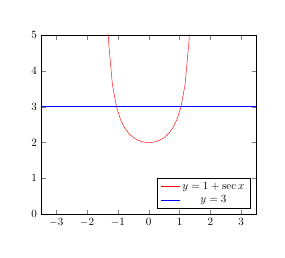
\begin{tikzpicture}[scale=0.4]
        \begin{axis}[ymin=0,ymax=5,xmin=-3.5,xmax=3.5,legend entries={$y=1+\sec x$, $y=3$},legend pos=south east]
\addplot [red,
domain=-pi/2:pi/2,
] {1+1/cos(deg(x))};
\addplot [blue,
domain=-4:4,
] {3};
\end{axis}
\end{tikzpicture}
\end{minipage}

\footnotesize
\pause
\begin{flalign*}
    V&=\int_{-\pi/3}^{\pi/3}\left(\pi(\textcolor{blue}3-1)^2 - \pi(\textcolor{red}{1+\sec x}-1)^2\right)\,dx=\pi\int_{-\pi/3}^{\pi/3}(4-\sec^2 x)\,dx\\
     &=\pi\left[4x-\tan x\right]_{-\pi/3}^{\pi/3}=\pi(4\pi/3-\sqrt3)-\pi(-4\pi/3+\sqrt3)=\boxed{\frac{8\pi^2}{3}-2\pi\sqrt3.}
\end{flalign*}
\pause (Note: we could have used symmetry to make the integral easier.)
\end{frame}

\begin{frame}{Volumes of solids of revolution (cylindrical shells)}
    Sometimes it is (much) easier to compute volumes of solids of revolution as follows.

    \vspace{2mm}
    \pause
    \textbf{Question}: find the volume of the solid of revolution obtained by rotating the region bounded by the curves $y=\sqrt{5+x^2}$, $y=0$, $x=0$ and $x=2$ around the $y$-axis.

    \vspace{2mm}
    \pause
    \textbf{Solution}: on the board (answer is $\frac23\pi(27-5^{3/2})$).
\end{frame}

\begin{frame}{Sample question (slide 1)}
    Let $f(x)=2xe^{2x}$.
    \begin{itemize}
        \item (a) Find the $x$- and $y$-coordinates of the local minima and maxima of $f(x)$.
        \item (b) Find the range of $f(x)$ for $-1\leq x\leq2$.
        \item (c) Find the area between the $x$-axis and the graph of $f(x)$ for $-1\leq x\leq 2$.
    \end{itemize}
    
\end{frame}

\begin{frame}{Sample question (slide 2)}

{\small Let $f(x)=2xe^{2x}$.
    \begin{itemize}
        \item (question a) Find the $x$- and $y$-coordinates of the local extrema of $f(x)$.
        \pause\item Solution: we compute the derivative $f'(x)=2e^{2x}+4xe^{2x}$ and set it to zero, so \begin{flalign*}
            2e^{2x}+4xe^{2x}=0\\
            2e^{2x}(1+2x)=0
        \end{flalign*}
        \pause
        Since $2e^{2x}$ is never equal to zero, our only solution to $f'(x)=0$ is $x=-\frac{1}{2}$. The corresponding $y$-coordinate is $f(-\frac{1}{2})=2(-\frac{1}{2})\cdot e^{2(-\frac{1}{2})}={-\frac{1}{e}}$.\pause

        We see that $f'(-1)=-2e^{-2}<0$ and $f'(0)=2>0$, so (by the first derivative test) we have a minimum, with coordinates $\boxed{{\left(-\frac{1}{2},-\frac{1}{e}\right)}}$. 
    \end{itemize}
}
\end{frame}

\begin{frame}{Sample question (slide 3)}
    Let $f(x)=2xe^{2x}$.
    \begin{itemize}
        \item (question b) Find the range of $f(x)$ for $-1\leq x\leq2$.
        \item\pause Solution: from question (a), we know that this function has a minimum with the coordinates $\left(-\frac{1}{2},-\frac{1}{e}\right)$. This minimum lies within the domain $-1\leq x\leq2$. \pause We are also interested in the value of $f(x)$ at the bounds of the domain, so we compute $f(-1)=-2e^{-2}$ and $f(2)=4e^4$. We observe that $-\frac{1}{e}<-2e^{-2}<4e^4$, so the range for $-1\leq x\leq2$ is $\boxed{\left[-\frac{1}{e},4e^4\right]}$.
    \end{itemize}
    
\end{frame}

\begin{frame}{Sample question (slide 4)}
    Let $f(x)=2xe^{2x}$.
    \begin{itemize}
        \item (question c) Find the area between the $x$-axis and the graph of $f(x)$ for $-1\leq x\leq 2$.
        \pause\item Solution: first compute the antiderivative of $f(x)$ using integration by parts: \[\int f(x)dx=\int2xe^{2x}dx=xe^{2x}-\int e^{2x}dx=\left(x-\frac{1}{2}\right)e^{2x}+C\]\pause
        
        We see that $f(x)$ is negative for $x<0$ and positive for $x>0$, so we have to split up the integral (we do not want ``negative area").\pause

        Our answer then becomes \[\hspace{-11mm}\left|\int_{-1}^0 f(x)dx\right|+\left|\int_{0}^{2} f(x)dx\right|=\left|-\frac{1}{2}+\frac{3}{2}e^{-2}\right|+\left|\frac{3}{2}e^4+\frac{1}{2}\right|=\boxed{1+\frac{3}{2}\left(e^4-e^{-2}\right)}\]
    \end{itemize}
    
\end{frame}
